\documentclass[aspectratio=169,xcolor=dvipsnames]{beamer}
\usetheme{SimpleDarkBlue}

\usepackage{hyperref}
\usepackage{graphicx}
\usepackage{booktabs}
\usepackage{amssymb}
\usepackage{amsmath}
\usepackage{tikz}
\usepackage{xcolor}
\usepackage{caption}
\usepackage{amsthm}

\title{Index Coding and Fractional Graph Theory}

\author{
	Mohammad Hosein Rabiee
	\and
	Amir Hosein Karimzadegan \\
}

\institute
{
	Department of Computer Science and Statistics \\
	Faculty of Mathematics \\
	K. N. Toosi University of Technology
}
\date{}

\begin{document}
	
	\begin{frame}
		\titlepage
	\end{frame}
	
	\begin{frame}{Index Coding Illustration}
		
		\begin{figure}
			\centering
			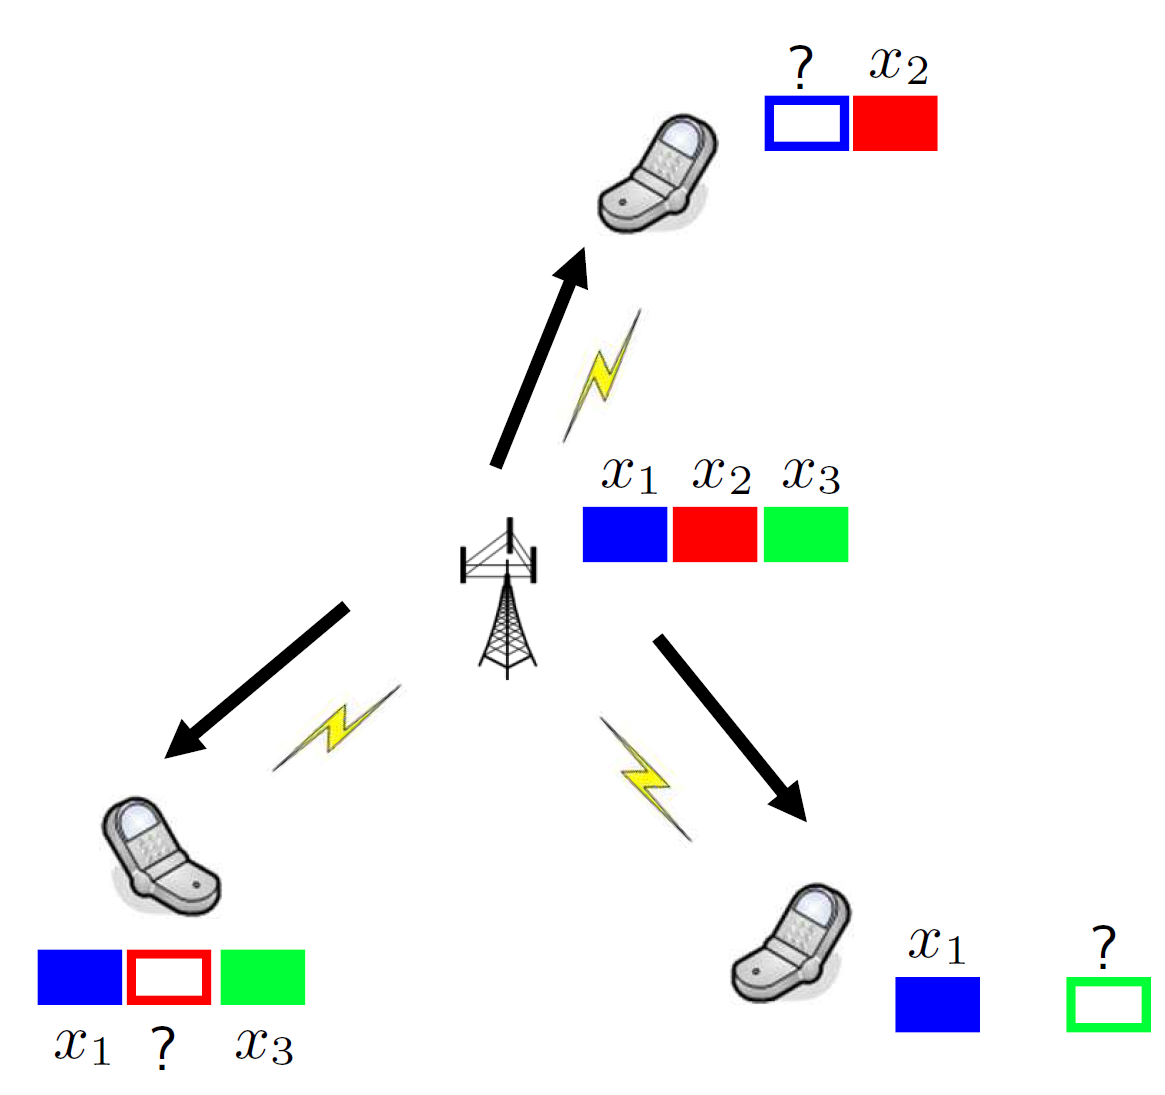
\includegraphics[width=0.4\linewidth]{images/indexcoding_illustration.png}
		\end{figure}
		\vspace{0.6em}
		
		\begin{itemize}[<+->]
			\item Send $x_1 + x_2$ and $x_3$
			\item What is the fundamental limit on the number of transmissions?
			\item Which coding scheme achieves the limit?
		\end{itemize}
		
	\end{frame}
	
	\begin{frame}{Representations}
		
		\begin{columns}[T]
			
			\column{0.55\textwidth}
			
			\begin{itemize}[<+->]
				\item \textbf{Side information}
				\[
				A_1 = \{2\}, \quad A_2 = \{1,3\}, \quad A_3 = \{1\}
				\]
				
				\item \textbf{Compact form}
				\[
				(1 \mid 2), \ (2 \mid 1,3), \ (3 \mid 1)
				\]
				
				\item \textbf{Side information graph $G$}
				
				\vspace{0.3em}
				\centering
				\includegraphics<3->[width=0.35\linewidth]{images/p1.png}
				
				\item <4-> \# of $n$-message index coding problems  
				$=$ \# of $n$-node directed graphs
				\[
				1,\, 3,\, 16,\, 218,\, 9608,\, 1540944,\, \ldots
				\]
				
				\item ``Equivalent'' to network coding  
				(Effros--El Rouayheb--Langberg, 2013)
			\end{itemize}
			
			\column{0.45\textwidth}
			\centering
			
			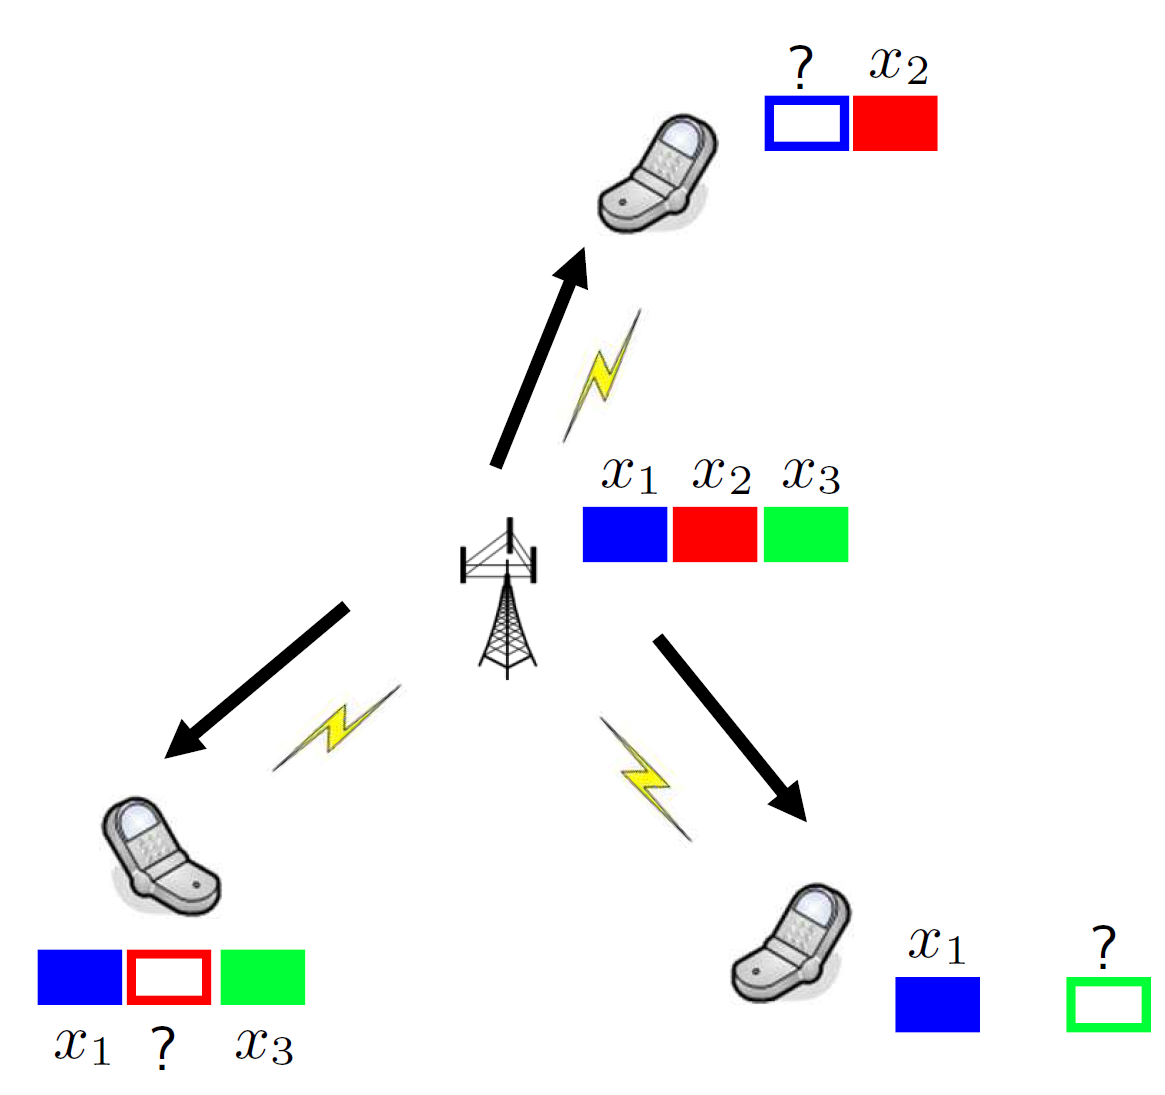
\includegraphics[width=0.65\linewidth]{images/indexcoding_illustration.png}
			
			\vspace{0.6em}
			
			\begin{itemize}
				\item<5-> \textbf{Multiple unicast network coding}
			\end{itemize}
			
			\vspace{0.4em}
			
			\includegraphics<5->[width=0.95\linewidth]{images/p2.png}
			
		\end{columns}
		
	\end{frame}
	
	\begin{frame}{Index coding}
		
		\vspace{-0.1cm}
		
		\begin{figure}
			\centering
			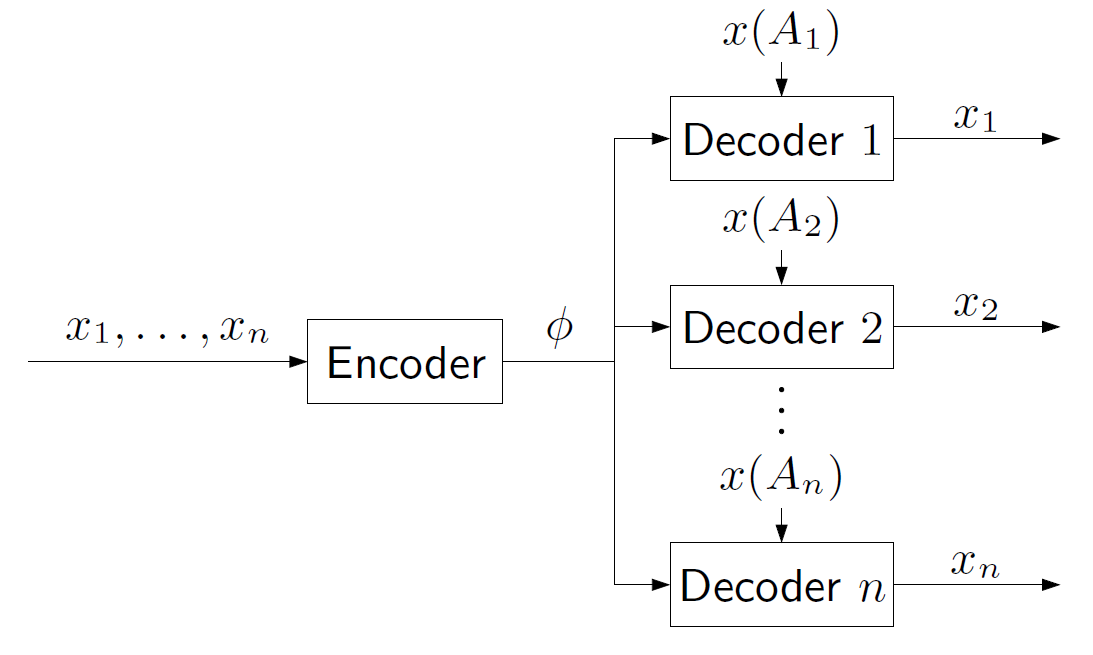
\includegraphics[width=0.5\linewidth]{images/p3.png}
		\end{figure}
		
		\vspace{0.4cm}
		
		\begin{itemize}
			\item $(t_1, \ldots, t_n, r)$ \textcolor{blue}{index code}
			
			\item\textcolor{blue}{Messages} $x_j \in \{0,1\}^{t_j}, \quad j \in [1:n]$
			
			\item\textcolor{blue}{Codeword} $\phi(x_1, \ldots, x_n) \in \{0,1\}^r$
			
			\item \textcolor{blue}{Side information}
			\[
			x(A_j) := (x_i : i \in A_j), 
			\quad A_j \subseteq [1:n] \setminus \{j\}
			\]
		\end{itemize}
		
	\end{frame}
	
	\begin{frame}{Achievability, Capacity region}
		
		\begin{block}{Achievability}
			\begin{itemize}
				\item A rate tuple $(R_1, \ldots, R_n)$ is \textcolor{blue}{achievable} iff there exists a
				$(t_1, \ldots, t_n, r)$ \textcolor{blue}{index code} such that
				\[
				R_j \le \frac{t_j}{r}, \quad j \in [1:n]
				\]
			\end{itemize}
		\end{block}
		
		\begin{block}{Capacity Region}
			\begin{itemize}
				\item The \textcolor{blue}{capacity region} $\mathcal{C}$ is the closure of the set of all
				achievable rate tuples.
			\end{itemize}
		\end{block}
		
		\begin{block}{Broadcast Rate}
			\begin{itemize}
				\item The \textcolor{blue}{broadcast rate} is defined as
				\[
				\beta = \min \left\{ b : \left(\tfrac{1}{b}, \ldots, \tfrac{1}{b}\right) \in \mathcal{C} \right\}
				\]
				\begin{itemize}
					\item $x_j \in \{0,1\}^{t}, \quad j \in [1:n], \quad 1 \le \beta \le n$
				\end{itemize}
			\end{itemize}
		\end{block}
		
	\end{frame}
	
	\begin{frame}{Outline}
		
		\begin{block}{Broadcast Rate}
			\begin{itemize}
				\item The \textcolor{blue}{broadcast rate} is defined as
				\[
				\beta = \min \left\{ b : \left(\tfrac{1}{b}, \ldots, \tfrac{1}{b}\right) \in \mathcal{C} \right\}
				\]
				\begin{itemize}
					\item $x_j \in \{0,1\}^{t}, \quad j \in [1:n], \quad 1 \le \beta \le n$
				\end{itemize}
			\end{itemize}
		\end{block}
		
		\begin{itemize}
			\item \textcolor{blue}{No computable characterization} of the capacity region $\mathcal{C}$
			or the broadcast rate $\beta$ in general.
			
			\item \textcolor{blue}{No approximation} within a factor of
			$O(n^{1-\varepsilon})$ for any $\varepsilon > 0$.
			
			\item \textcolor{blue}{Existing results}
			\begin{itemize}
				\item \textcolor{blue}{Lower bounds} on the broadcast rate $\beta$
				\item \textcolor{blue}{Coding schemes} (upper bounds on $\beta$)
			\end{itemize}
		\end{itemize}
		
	\end{frame}
	
	\begin{frame}{Cycle-free bound}
		
		\begin{columns}[c]
			
			\column{0.4\textwidth}
			\centering
			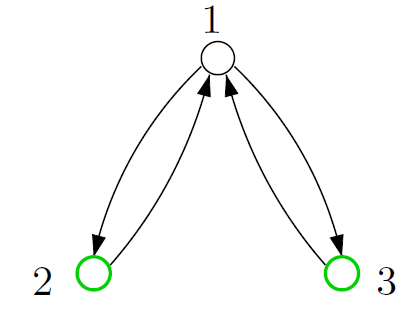
\includegraphics[width=0.6\linewidth]{images/c1.png}
			
			\vspace{0.4em}
			\[
			2 = \alpha(G) \le \beta
			\]
			
			\column{0.4\textwidth}
			\centering
			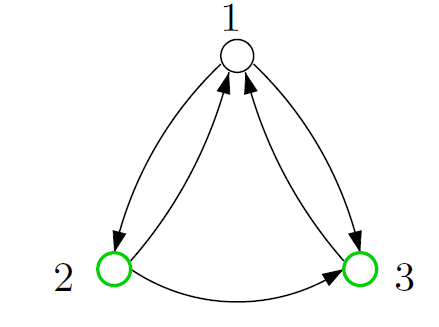
\includegraphics[width=0.6\linewidth]{images/c2.png}
			
			\vspace{0.1em}
			\[
			2 \le \beta
			\]
			
		\end{columns}
		
		\vspace{1em}
		
		\begin{block}{Cycle-free lower bound(Neely--Tehrani--Zhang 2013)}
			\[
			\max_{S \subseteq [1:n] \,:\, G|_S \text{ is cycle-free}} |S| \;\le\; \beta
			\]
		\end{block}
		
	\end{frame}
	
	\begin{frame}{Polymatroidal outer bound}
		
		\begin{block}{Polymatroidal bound (Dougherty et al.\ 2011, Blasiak et al.\ 2011)}
			
			If $(R_1,\ldots,R_n)$ is achievable for the index coding problem $(j \mid A_j)$,
			$j \in [1:n]$, then
			\[
			R_j \le f(B_j \cup \{j\}) - f(B_j), \qquad j \in [1:n],
			\]
			for some set function $f$ such that
			\begin{itemize}
				\item $f(\emptyset) = 0$
				\item $f([1:n]) = 1$
				\item $f(J) \le f(K), \qquad J \subseteq K \subseteq [1:n]$
				\item $f(J \cap K) + f(J \cup K) \le f(J) + f(K), \qquad J,K \subseteq [1:n]$
			\end{itemize}
			
		\end{block}
		
		\vspace{0.8em}
		
		\begin{itemize}
			\item Proof based on \textcolor{blue}{submodularity of entropy}
			\item Tighter than the \textcolor{blue}{cycle-free bound}
			\item Not tight (Sun--Jafar 2013)
		\end{itemize}
		
	\end{frame}
	
	\begin{frame}{Overview of coding schemes}
		
		\begin{figure}
			\centering
			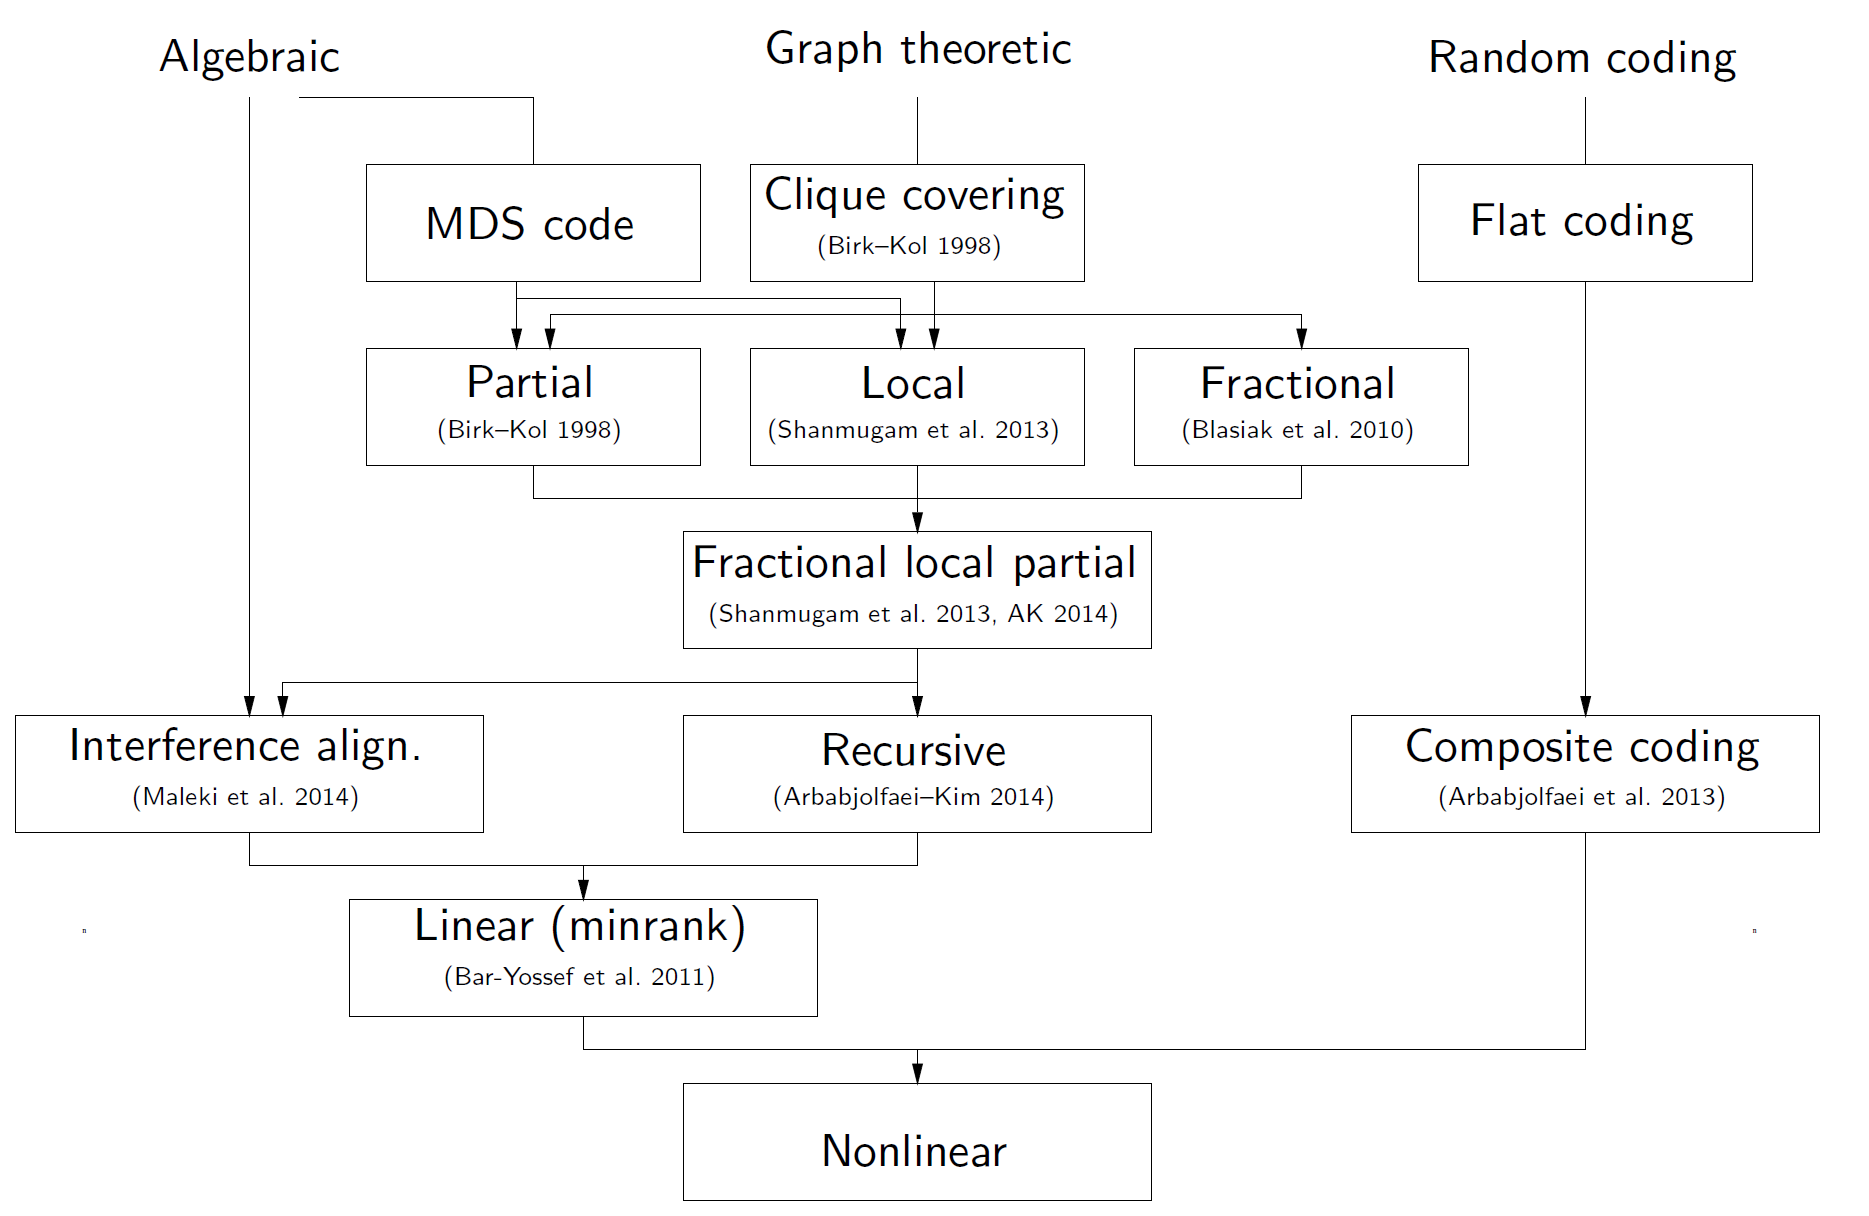
\includegraphics[width=0.8\linewidth]{images/p4.png}
		\end{figure}
		
	\end{frame}
	
	\begin{frame}{MDS Code}
		
		\begin{itemize}
			\item \textcolor{blue}{Side information pattern}:
			\[
			(1 \mid 2), \ (2 \mid 1,3), \ (3 \mid 1)
			\]
			
			\item Every node has at least \textcolor{blue}{one piece of side information}.
			
			\item \textcolor{blue}{Systematic $(5,3)$ MDS code}:
			\[
			(x_1, x_2, x_3, p_1, p_2)
			\]
			
			\item Sending only the \textcolor{blue}{parity symbols} achieves
			\[
			\beta = 2.
			\]
			
			\item In general,
			\[
			\beta = |V| - \min_{v \in V} \text{indegree}(v).
			\]
			
			\item The \textcolor{blue}{partial clique number}
			\[
			\kappa(G) = |V| - \min_{v \in V} \text{indegree}(v).
			\]
			
			\item If the side information graph is a \textcolor{blue}{clique}, then
			\[
			\beta = 1.
			\]
		\end{itemize}
		
	\end{frame}
	
	\begin{frame}{Representing the Problem}
		Before we can optimize, we must model the system as a directed graph $G(V, E)$.
		
		\vspace{1em}
		
		\begin{columns}[c]
			\column{0.6\textwidth}
			\textbf{Graph Construction Rules:}
			\begin{enumerate}
				\item \textbf{Nodes ($V$):} Each node represents a Receiver (who wants a specific message $x_i$).
				\item \textbf{Edges ($E$):} A directed edge $(i, j)$ exists if Receiver $i$ \textbf{HAS} message $x_j$ (Side Information).
			\end{enumerate}
			
			\vspace{1em}
			\begin{block}{Key Takeaway}
				The more edges we have (more side information), the fewer transmissions we need. Our goal is to exploit the structure of these edges.
			\end{block}
			
			\column{0.4\textwidth}
			\centering
			\Huge $G = (V, E)$
			\vspace{0.5em}
			\normalsize
			\\ \textit{Side Information Graph}
		\end{columns}
	\end{frame}
	
	\begin{frame}{Clique Covering: The Intuition}
		\begin{columns}[c]
			\column{.55\textwidth}
			\begin{block}{The Concept}
				Now, let's look at a specific structure: A \alert{Clique}. This is when a group of receivers all know each other's desired messages.
			\end{block}
			\vspace{0.5em}
			\begin{itemize}
				\item \textbf{Scenario:}
				\begin{itemize}
					\item Receiver 1 wants $x_1$, has $x_2$.
					\item Receiver 2 wants $x_2$, has $x_1$.
				\end{itemize}
				\item \textbf{Solution:} Broadcast \textcolor{blue}{XOR sum} ($x_1 \oplus x_2$).
				\item \textbf{Result:}
				\begin{itemize}
					\item $R_1$: $(x_1 \oplus x_2) \oplus x_2 \to x_1$
					\item $R_2$: $(x_1 \oplus x_2) \oplus x_1 \to x_2$
				\end{itemize}
				\item \textbf{Cost:} 1 Transmission for 2 Users.
			\end{itemize}
			
			\column{.45\textwidth}
			\begin{figure}
				\centering
				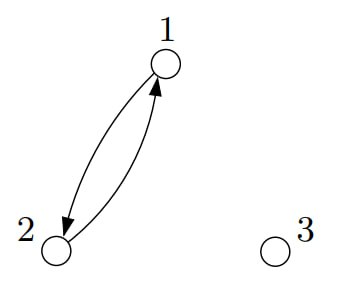
\includegraphics[width=0.9\linewidth]{images/cliqe_2.jpg}
				\caption{Perfect Clique}
			\end{figure}
		\end{columns}
	\end{frame}
	
	\begin{frame}{Method 1: Clique Partitioning}
		\begin{columns}[c]
			\column{.55\textwidth}
			\begin{alertblock}{The Strategy}
				Partition the entire graph into the \textbf{minimum number of cliques}.
			\end{alertblock}
			\vspace{0.8em}
			\textbf{In this example:}
			\begin{enumerate}
				\item Nodes 1 \& 2 form a clique $\to$ Cost: 1.
				\item Node 3 is isolated $\to$ Cost: 1.
			\end{enumerate}
			\vspace{0.5em}
			\begin{itemize}
				\item \textbf{Rate ($b$):} Equal to the \textcolor{blue}{Clique Cover Number} of the graph.
				\item \textbf{Limit:} This requires bidirectional knowledge (edges going both ways).
			\end{itemize}
			
			\column{.45\textwidth}
			\begin{figure}
				\centering
				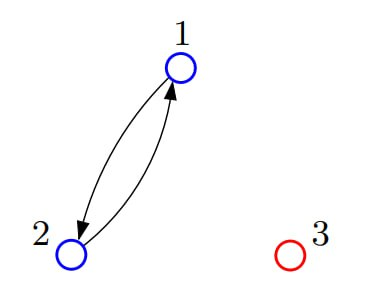
\includegraphics[width=0.9\linewidth]{images/cliqe_1.jpg}
			\end{figure}
		\end{columns}
	\end{frame}
	
	\begin{frame}{The Limitation: The Cycle Problem}
		\begin{columns}[c]
			\column{.55\textwidth}
			\begin{block}{The Issue}
				Strict Clique Covering ignores "partial" knowledge.
			\end{block}
			
			\textbf{Look at the cycle (1-2-3):}
			\begin{itemize}
				\item 1 has 2; 2 has 3; 3 has 1.
				\item This is \textbf{NOT} a clique (edges are one-way).
			\end{itemize}
			
			\vspace{0.5em}
			\textbf{Inefficiency:}
			\begin{itemize}
				\item Standard clique algorithms treat these as separate nodes.
				\item \textbf{Naive Cost:} 3 Transmissions (One for each).
				\item We need a method that handles cycles.
			\end{itemize}
			
			\column{.45\textwidth}
			\begin{figure}
				\centering
				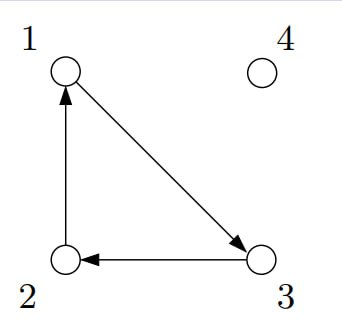
\includegraphics[width=0.9\linewidth]{images/cliqe_3.jpg}
				\caption{Directed Cycle (No Cliques)}
			\end{figure}
		\end{columns}
	\end{frame}
	
	\begin{frame}{Method 2: Partial Clique Covering}
		\begin{columns}[c]
			\column{.55\textwidth}
			\begin{alertblock}{The Solution}
				\textcolor{blue}{Partial Clique Covering} relaxes the requirement. We group nodes based on "missing" info.
			\end{alertblock}
			\vspace{0.5em}
			\begin{itemize}
				\item We treat the cycle (1, 2, 3) as a single group (Blue).
				\item Instead of simple XOR, we use \textbf{Linear Coding}.
				\item \textbf{Result:} We can service 3 users with fewer than 3 transmissions.
				\item This is equivalent to \textbf{Fractional Graph Coloring}.
			\end{itemize}
			
			\column{.45\textwidth}
			\begin{figure}
				\centering
				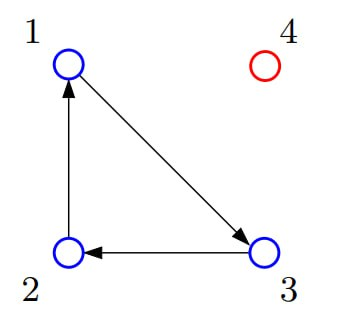
\includegraphics[width=0.9\linewidth]{images/cliqe_4.jpg}
				\caption{Partial Clique Grouping}
			\end{figure}
		\end{columns}
	\end{frame}
	
	\begin{frame}{Real Example: Solving the Cycle}
		Let's solve the Cycle (1-2-3) using just \textbf{2 transmissions} for 3 users.
		
		\begin{columns}[t]
			\column{0.45\textwidth}
			\textbf{1. The Setup (What users have):}
			\begin{itemize}
				\item $R_1$: Wants $x_1$, Has $x_2$
				\item $R_2$: Wants $x_2$, Has $x_3$
				\item \textbf{$R_3$: Wants $x_3$, Has $x_1$}
			\end{itemize}
			
			\vspace{1em}
			\textbf{2. The Transmissions (Server):}
			We broadcast two linear sums:
			$$ L_1 = x_1 + x_2 $$
			$$ L_2 = x_2 + x_3 $$
			
			\column{0.5\textwidth}
			\textbf{3. Decoding (Perspective of $R_3$):}
			\\ \small{$R_3$ receives $L_1$ and $L_2$. $R_3$ only knows $x_1$.}
			
			\vspace{0.5em}
			\begin{block}{Step-by-Step Recovery}
				\begin{enumerate}
					\item Take $L_1$ and subtract known $x_1$:
					$$ (x_1 + x_2) - \mathbf{x_1} = \mathbf{x_2} $$
					\item Now $R_3$ knows $x_2$!
					\item Take $L_2$ and subtract newly found $x_2$:
					$$ (x_2 + x_3) - \mathbf{x_2} = \mathbf{x_3} $$
				\end{enumerate}
			\end{block}
			\vspace{0.2em}
			\centering \textcolor{green}{\textbf{Success! $R_3$ recovered $x_3$.}}
		\end{columns}
	\end{frame}
	
	\begin{frame}
		\Huge{\centerline{\textbf{Thank you!}}}
	\end{frame}
	
\end{document}
